\documentclass{zkdl-presentation-template}

\usepackage[T1]{fontenc}
\usepackage{kerkis}
\usepackage{kmath}
%\usepackage{concmath}
\usepackage{centernot}

\newcommand\leftarrowS{\leftarrow\joinrel\smalldollar}
\newcommand\rightarrowS{\smalldollar\joinrel\rightarrow}

\makeatletter
\newcommand{\smalldollar}{\mathrel{\mathpalette\small@dollar\relax}}
\newcommand{\small@dollar}[2]{%
  \vcenter{\hbox{%
    $#1\textnormal{\fontsize{0.7\dimexpr\f@size pt}{0}\selectfont\$}$%
  }}%
}
\makeatother

\tikzset{
    grid_cell/.style={
        rectangle, 
        draw=black, 
        very thick,
        minimum size=0.75cm, 
        font=\large\bfseries
    },
    grid_label/.style={
        font=\small
    },
    hypercube_highlight/.style={
        fill=gray!40
    }
}

% Define values for x_1 to x_8
\newcommand{\xval}[1]{%
\ifcase#1
    % case 0 (won't be used)
    \or 1  % 1st
    \or 2  % 2nd
    \or 0  % 3rd
    \or 1  % 4th
    \or 0  % 5th
    \or 2  % 6th
    \or 0  % 7th
    \or 1  % 8th
\fi
}

\title[GKR \& Memory Checking]{\textbf{GKR Protocol. Offline Memory Checking}}
\author{Distributed Lab}
\date{July 17, 2025}
\homepage{zkdl-camp.github.io}
\github{ZKDL-Camp}

\begin{document}
    \frame {
        \tikz [remember picture,overlay]
        \node at
            ([yshift=1.5cm,xshift=-1.5cm]current page.south east) 
            %or: (current page.center)
            {
\includegraphics[width=60pt]{images/logo.png}};
        \titlepage
    }

	\section{Introduction}

    \begin{frame}{Recap: Multivariate World and Sum-Check}
        \begin{figure}
            \centering
            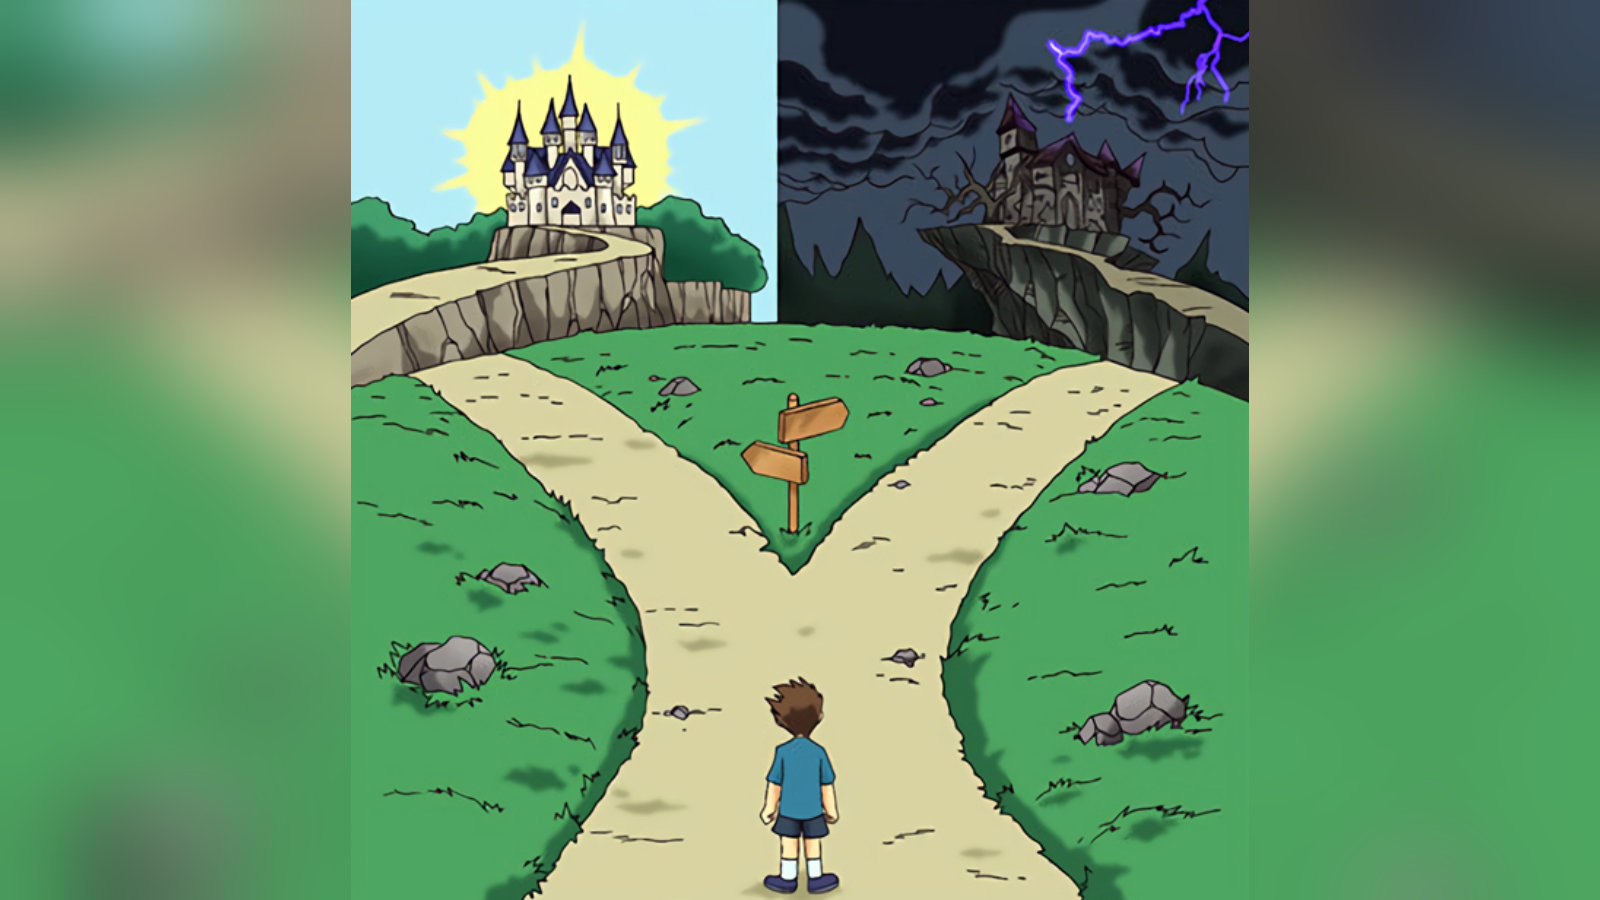
\includegraphics[width=0.55\textwidth]{images/lecture_15/bad_boy.jpg}
        \end{figure}
        \begin{columns}
            \begin{column}{0.5\textwidth}
                \textcolor{blue!70!black}{\begin{center}
                    \textbf{Univariate World:}
                \end{center}
                \[p(X) = q(X)\prod_{u \in \Omega}(X-u)\]}
            \end{column}
            \begin{column}{0.5\textwidth}
                \textcolor{green!50!black}{
                \begin{center}
                    \textbf{Multivariate World:}
                \end{center}
                \[\sum_{\mathbf{b} \in \{0,1\}^{\ell}} f(b_1,\dots,b_{\ell}) = H\]}
            \end{column}
        \end{columns}

        \vspace{-10px}
        
        \textbf{Goal:} build the set of constraints that boil down to \textbf{Sum-Check}:
        \begin{equation*}
            \textcolor{green!50!black}{\sum_{(b_1,\dots,b_{\ell}) \in \{0,1\}^{\ell}} f(b_1,\dots,b_{\ell}) = H}
        \end{equation*}

        \textbf{Cost:} Quasilinear prover, logarithmic verifier and proof size.
    \end{frame}

    \section{GKR Protocol}

    \begin{frame}{Motivation}
        \textcolor{blue!70!black}{\textbf{Goal:} Build sumcheck-based version of the circuit
        arithmetization.}

        Suppose we are given the \textbf{layered} fan-in two arithmetical
        circuit $\mathtt{C}: \mathbb{F}^n \to \mathbb{F}^m$ of size $S$ (number
        of gates). The \textit{layered} here means that the circuit $\mathtt{C}$
        can be decomposed into $d$ layers (note that GKR can be generalized to
        the unstructured arithmetical circuits as well). 
        \begin{figure}
            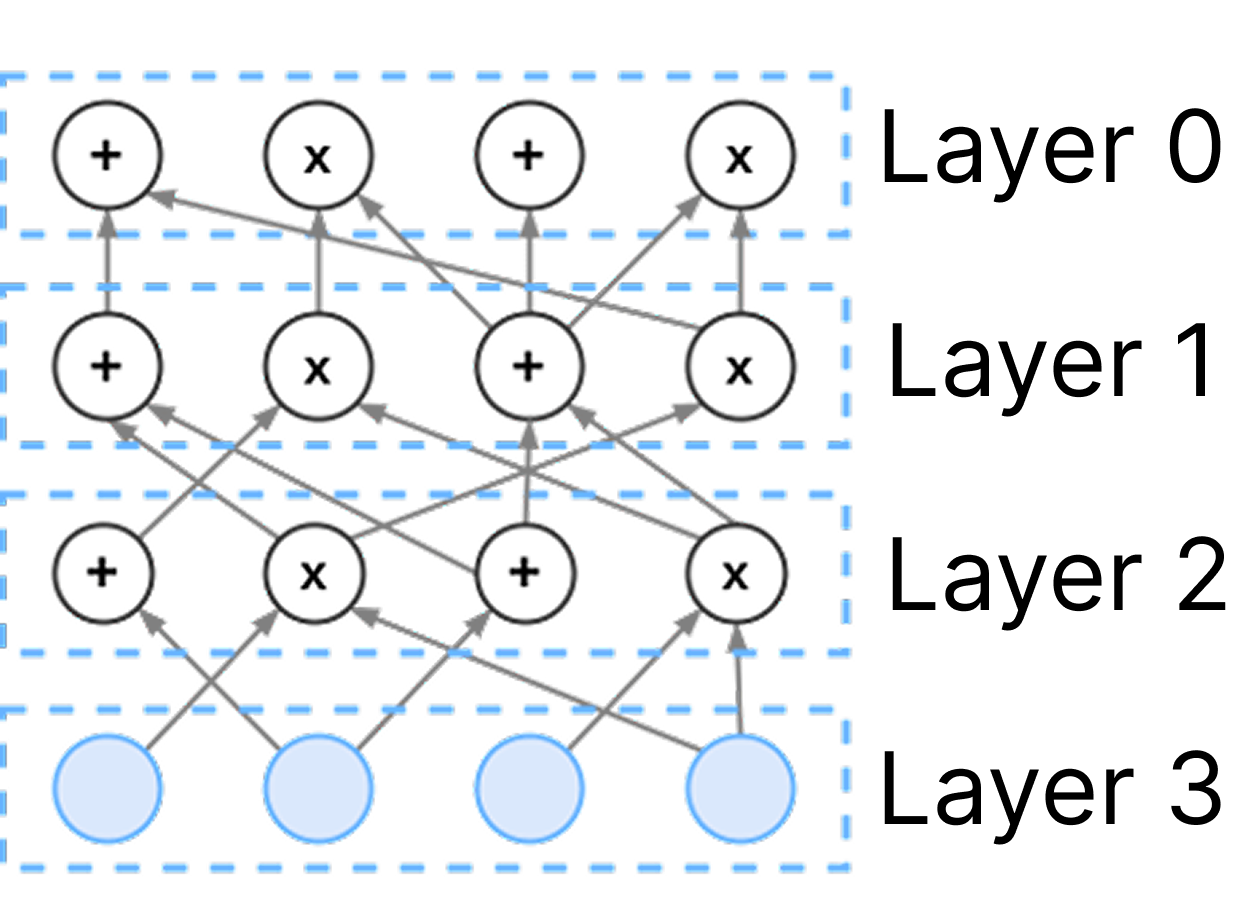
\includegraphics[width=0.5\linewidth]{images/lecture_16/structured.png}
            \caption{Layered Circuit Structure of $d=4$ layers.}
        \end{figure}
    \end{frame}

    \begin{frame}{Spoilers on Performance}        
        The GKR protocol allows 
        to achieve the following performance:
        \begin{itemize}
            \item The communication consists of $\mathcal{O}(d \cdot \mathsf{polylog}(S))$ field elements.
            \item The verifier runs in $\mathcal{O}(n + d \cdot \mathsf{polylog}(S))$ time.
            \item The prover runs in $\mathcal{O}(\mathsf{poly}(S))$ time.
            \item The soundness error is just $\mathcal{O}(d \log(S) / |\mathbb{F}|)$.
        \end{itemize}

        \textbf{Assumptions:}
        \begin{itemize}
            \item Assume we have $d$ rounds in total. Output layer is the
            $0^{\text{th}}$ layer.
            \item Each layer consists of $S_i$ gates.
            \item Assume $S_i=2^{v_i}$ is the power of two
        \end{itemize}
    \end{frame}

    \begin{frame}{Concrete Circuit}
        \begin{figure}[H]
        \centering
        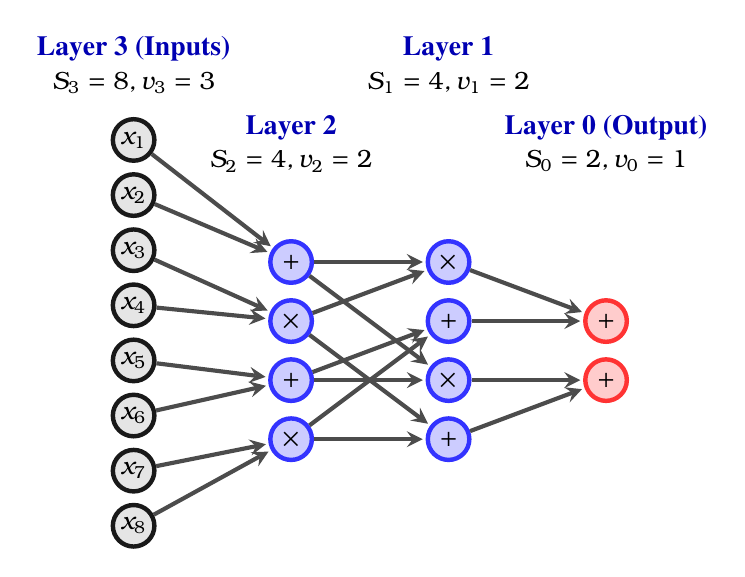
\begin{tikzpicture}[
            % Define styles for different parts of the circuit
            input/.style={circle, ultra thick, draw=gray!20!black, fill=gray!20, minimum size=15pt, inner sep=0pt},
            gate/.style={circle, ultra thick, draw=blue!80, fill=blue!20, minimum size=15pt, inner sep=0pt},
            output/.style={circle, ultra thick, draw=red!80, fill=red!20, minimum size=15pt, inner sep=0pt},
            conn/.style={-stealth, draw=black!70, shorten >=1pt, line width=1.5pt}
        ]

        % --- Layer Labels ---
        \node[font=\bfseries, align=center] at (0, 7.75) {\textcolor{blue!70!black}{Layer 3 (Inputs)} \\ $S_3=8,v_3=3$};
        \node[font=\bfseries, align=center] at (2, 6.75) {\textcolor{blue!70!black}{Layer 2}\\ $S_2=4,v_2=2$};
        \node[font=\bfseries, align=center] at (4, 7.75) {\textcolor{blue!70!black}{Layer 1} \\ $S_1=4,v_1=2$};
        \node[font=\bfseries, align=center] at (6, 6.75) {\textcolor{blue!70!black}{Layer 0 (Output)} \\ $S_0=2, v_0=1$};


        % --- Layer 0: Input Nodes (8) ---
        % We use a \foreach loop to create the 8 input nodes vertically
        \foreach \i in {1,...,8} {
            \node[input] (l0-\i) at (0, 7.5 - 0.7*\i) {$x_{\i}$};
        }

        % --- Layer 1: Gate Nodes (4) ---
        % Alternating between + and x gates
        \node[gate] (l1-1) at (2, 5.25) {$+$};
        \node[gate] (l1-2) at (2, 4.5) {$\times$};
        \node[gate] (l1-3) at (2, 3.75) {$+$};
        \node[gate] (l1-4) at (2, 3.0) {$\times$};

        % --- Layer 2: Gate Nodes (4) ---
        \node[gate] (l2-1) at (4, 5.25) {$\times$};
        \node[gate] (l2-2) at (4, 4.5) {$+$};
        \node[gate] (l2-3) at (4, 3.75) {$\times$};
        \node[gate] (l2-4) at (4, 3.0) {$+$};

        % --- Layer 3: Output Nodes (2) ---
        \node[output] (l3-1) at (6, 4.5) {$+$};
        \node[output] (l3-2) at (6, 3.75) {$+$};


        % --- Connections ---

        % Connections from Layer 0 to Layer 1
        \foreach \i in {1,...,4} {
            \pgfmathtruncatemacro{\j}{2 * \i - 1} % Calculate first source node index
            \pgfmathtruncatemacro{\k}{2 * \i}     % Calculate second source node index
            \draw[conn] (l0-\j) -- (l1-\i);
            \draw[conn] (l0-\k) -- (l1-\i);
        }

        % Connections from Layer 1 to Layer 2
        % This wiring pattern creates a mixing of the signals
        \draw[conn] (l1-1) -- (l2-1);
        \draw[conn] (l1-2) -- (l2-1);

        \draw[conn] (l1-3) -- (l2-2);
        \draw[conn] (l1-4) -- (l2-2);

        \draw[conn] (l1-1) -- (l2-3);
        \draw[conn] (l1-3) -- (l2-3);

        \draw[conn] (l1-2) -- (l2-4);
        \draw[conn] (l1-4) -- (l2-4);

        % Connections from Layer 2 to Layer 3
        \draw[conn] (l2-1) -- (l3-1);
        \draw[conn] (l2-2) -- (l3-1);

        \draw[conn] (l2-3) -- (l3-2);
        \draw[conn] (l2-4) -- (l3-2);

        \end{tikzpicture}
        \caption{Example layered arithmetical circuit $\mathtt{C}: \mathbb{F}^8 \to
        \mathbb{F}^2$ with $d=3$ layers.}
        \end{figure}
    \end{frame}

    \begin{frame}{Gates Encoding}
        \textcolor{blue!70!black}{\textbf{Gates Encoding.}} Suppose $W_i: \{0,1\}^{v_i} \to \mathbb{F}$ is
        structured so that it outputs the value of the $i$-th layer gate given the gate
        label. Assume MLE of $W_i$ is
        $\widetilde{W}_i: \mathbb{F}^{v_i} \to \mathbb{F}$.

        \begin{center}
        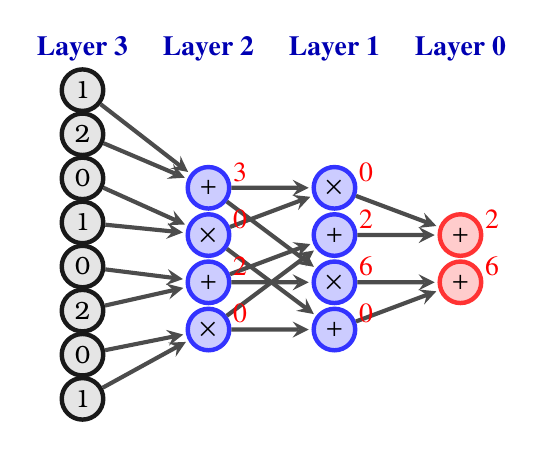
\begin{tikzpicture}[
            % Define styles for different parts of the circuit
            input/.style={circle, ultra thick, draw=gray!20!black, fill=gray!20, minimum size=15pt, inner sep=0pt},
            gate/.style={circle, ultra thick, draw=blue!80, fill=blue!20, minimum size=15pt, inner sep=0pt},
            output/.style={circle, ultra thick, draw=red!80, fill=red!20, minimum size=15pt, inner sep=0pt},
            conn/.style={-stealth, draw=black!70, shorten >=1pt, line width=1.5pt},
            scale=0.8
        ]

        % --- Layer Labels ---
        \node[font=\bfseries, align=center] at (0, 7.45) {\textcolor{blue!70!black}{Layer 3}};
        \node[font=\bfseries, align=center] at (2, 7.45) {\textcolor{blue!70!black}{Layer 2}};
        \node[font=\bfseries, align=center] at (4, 7.45) {\textcolor{blue!70!black}{Layer 1}};
        \node[font=\bfseries, align=center] at (6, 7.45) {\textcolor{blue!70!black}{Layer 0}};

        % --- Layer 0: Input Nodes (8) ---
        % We use a \foreach loop to create the 8 input nodes vertically
        \foreach \i in {1,...,8} {
            \node[input] (l0-\i) at (0, 7.5 - 0.7*\i) {$\xval{\i}$};
        }

        % --- Layer 1: Gate Nodes (4) ---
        % Alternating between + and x gates
        \node[gate] (l1-1) at (2, 5.25) {$+$};

        \node[gate] (l1-2) at (2, 4.5) {$\times$};
 
        \node[gate] (l1-3) at (2, 3.75) {$+$};

        \node[gate] (l1-4) at (2, 3.0) {$\times$};

        % --- Layer 2: Gate Nodes (4) ---
        \node[gate] (l2-1) at (4, 5.25) {$\times$};
        \node[gate] (l2-2) at (4, 4.5) {$+$};
        \node[gate] (l2-3) at (4, 3.75) {$\times$};
        \node[gate] (l2-4) at (4, 3.0) {$+$};

        % --- Layer 3: Output Nodes (2) ---
        \node[output] (l3-1) at (6, 4.5) {$+$};
        \node[output] (l3-2) at (6, 3.75) {$+$};


        % --- Connections ---

        % Connections from Layer 0 to Layer 1
        \foreach \i in {1,...,4} {
            \pgfmathtruncatemacro{\j}{2 * \i - 1} % Calculate first source node index
            \pgfmathtruncatemacro{\k}{2 * \i}     % Calculate second source node index
            \draw[conn] (l0-\j) -- (l1-\i);
            \draw[conn] (l0-\k) -- (l1-\i);
        }

        % Connections from Layer 1 to Layer 2
        % This wiring pattern creates a mixing of the signals
        \draw[conn] (l1-1) -- (l2-1);
        \draw[conn] (l1-2) -- (l2-1);

        \draw[conn] (l1-3) -- (l2-2);
        \draw[conn] (l1-4) -- (l2-2);

        \draw[conn] (l1-1) -- (l2-3);
        \draw[conn] (l1-3) -- (l2-3);

        \draw[conn] (l1-2) -- (l2-4);
        \draw[conn] (l1-4) -- (l2-4);

        % Connections from Layer 2 to Layer 3
        \draw[conn] (l2-1) -- (l3-1);
        \draw[conn] (l2-2) -- (l3-1);

        \draw[conn] (l2-3) -- (l3-2);
        \draw[conn] (l2-4) -- (l3-2);

        % Values in gates, layer 2
        \node at (2.5, 5.5) {\textcolor{red}{3}};
        \node at (2.5, 4.75) {\textcolor{red}{0}};
        \node at (2.5, 4.0) {\textcolor{red}{2}};
        \node at (2.5, 3.25) {\textcolor{red}{0}};

        % Values in gates, layer 1
        \node at (4.5, 5.5) {\textcolor{red}{0}};
        \node at (4.5, 4.75) {\textcolor{red}{2}};
        \node at (4.5, 4.0) {\textcolor{red}{6}};
        \node at (4.5, 3.25) {\textcolor{red}{0}};

        % Values in gates, layer 0
        \node at (6.5, 4.75) {\textcolor{red}{2}};
        \node at (6.5, 4.0) {\textcolor{red}{6}};
        \end{tikzpicture}
        \end{center}
        \vspace{-12.5px}
        \begin{gather*}
            W_1(0, 0) = 0, \quad W_1(0, 1) = 2, \quad W_1(1, 0) = 6, \quad W_1(1, 1) = 0 \\
            \textbf{MLE Extension:} \quad \widetilde{W}_1(X_1,X_2) = 2(1-X_1)X_2 + 6X_1(1-X_2)
        \end{gather*}
    \end{frame}

    \begin{frame}{Wiring Encoding}
        \textcolor{green!80!black}{\textbf{Wiring Predicates.}} $\mathsf{in}_{1,i}, \mathsf{in}_{2,i}:
        \{0,1\}^{v_i} \to \{0,1\}^{v_{i+1}}$ indicate which pairs of
        wiring are connected to the $i^{\text{th}}$ layer gate from the layer $i+1$.

        \begin{center}
        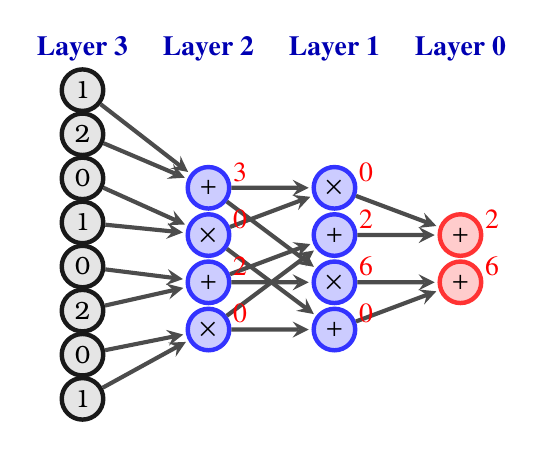
\begin{tikzpicture}[
            % Define styles for different parts of the circuit
            input/.style={circle, ultra thick, draw=gray!20!black, fill=gray!20, minimum size=15pt, inner sep=0pt},
            gate/.style={circle, ultra thick, draw=blue!80, fill=blue!20, minimum size=15pt, inner sep=0pt},
            output/.style={circle, ultra thick, draw=red!80, fill=red!20, minimum size=15pt, inner sep=0pt},
            conn/.style={-stealth, draw=black!70, shorten >=1pt, line width=1.5pt},
            scale=0.8
        ]

        % --- Layer Labels ---
        \node[font=\bfseries, align=center] at (0, 7.45) {\textcolor{blue!70!black}{Layer 3}};
        \node[font=\bfseries, align=center] at (2, 7.45) {\textcolor{blue!70!black}{Layer 2}};
        \node[font=\bfseries, align=center] at (4, 7.45) {\textcolor{blue!70!black}{Layer 1}};
        \node[font=\bfseries, align=center] at (6, 7.45) {\textcolor{blue!70!black}{Layer 0}};

        % --- Layer 0: Input Nodes (8) ---
        % We use a \foreach loop to create the 8 input nodes vertically
        \foreach \i in {1,...,8} {
            \node[input] (l0-\i) at (0, 7.5 - 0.7*\i) {$\xval{\i}$};
        }

        % --- Layer 1: Gate Nodes (4) ---
        % Alternating between + and x gates
        \node[gate] (l1-1) at (2, 5.25) {$+$};

        \node[gate] (l1-2) at (2, 4.5) {$\times$};
 
        \node[gate] (l1-3) at (2, 3.75) {$+$};

        \node[gate] (l1-4) at (2, 3.0) {$\times$};

        % --- Layer 2: Gate Nodes (4) ---
        \node[gate] (l2-1) at (4, 5.25) {$\times$};
        \node[gate] (l2-2) at (4, 4.5) {$+$};
        \node[gate] (l2-3) at (4, 3.75) {$\times$};
        \node[gate] (l2-4) at (4, 3.0) {$+$};

        % --- Layer 3: Output Nodes (2) ---
        \node[output] (l3-1) at (6, 4.5) {$+$};
        \node[output] (l3-2) at (6, 3.75) {$+$};


        % --- Connections ---

        % Connections from Layer 0 to Layer 1
        \foreach \i in {1,...,4} {
            \pgfmathtruncatemacro{\j}{2 * \i - 1} % Calculate first source node index
            \pgfmathtruncatemacro{\k}{2 * \i}     % Calculate second source node index
            \draw[conn] (l0-\j) -- (l1-\i);
            \draw[conn] (l0-\k) -- (l1-\i);
        }

        % Connections from Layer 1 to Layer 2
        % This wiring pattern creates a mixing of the signals
        \draw[conn] (l1-1) -- (l2-1);
        \draw[conn] (l1-2) -- (l2-1);

        \draw[conn] (l1-3) -- (l2-2);
        \draw[conn] (l1-4) -- (l2-2);

        \draw[conn] (l1-1) -- (l2-3);
        \draw[conn] (l1-3) -- (l2-3);

        \draw[conn] (l1-2) -- (l2-4);
        \draw[conn] (l1-4) -- (l2-4);

        % Connections from Layer 2 to Layer 3
        \draw[conn] (l2-1) -- (l3-1);
        \draw[conn] (l2-2) -- (l3-1);

        \draw[conn] (l2-3) -- (l3-2);
        \draw[conn] (l2-4) -- (l3-2);

        % Values in gates, layer 2
        \node at (2.5, 5.5) {\textcolor{red}{3}};
        \node at (2.5, 4.75) {\textcolor{red}{0}};
        \node at (2.5, 4.0) {\textcolor{red}{2}};
        \node at (2.5, 3.25) {\textcolor{red}{0}};

        % Values in gates, layer 1
        \node at (4.5, 5.5) {\textcolor{red}{0}};
        \node at (4.5, 4.75) {\textcolor{red}{2}};
        \node at (4.5, 4.0) {\textcolor{red}{6}};
        \node at (4.5, 3.25) {\textcolor{red}{0}};

        % Values in gates, layer 0
        \node at (6.5, 4.75) {\textcolor{red}{2}};
        \node at (6.5, 4.0) {\textcolor{red}{6}};
        \end{tikzpicture}
        \end{center}
    \end{frame}

    \begin{frame}{Wiring Encoding}
        \textcolor{green!80!black}{\textbf{Wiring Predicates.}} $\mathsf{in}_{1,i}, \mathsf{in}_{2,i}:
        \{0,1\}^{v_i} \to \{0,1\}^{v_{i+1}}$ indicate which pairs of
        wiring are connected to the $i^{\text{th}}$ layer gate from the layer $i+1$.

        \begin{center}
        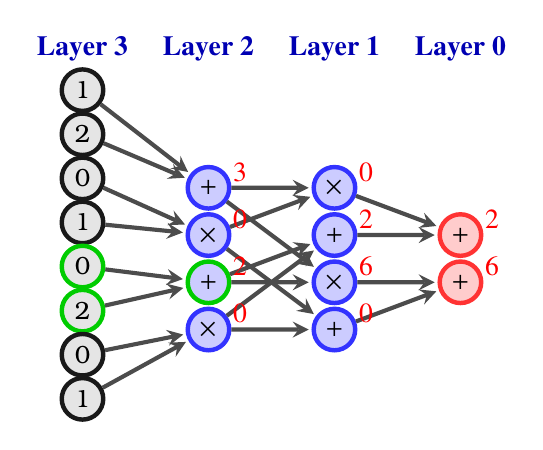
\begin{tikzpicture}[
            % Define styles for different parts of the circuit
            input/.style={circle, ultra thick, draw=gray!20!black, fill=gray!20, minimum size=15pt, inner sep=0pt},
            gate/.style={circle, ultra thick, draw=blue!80, fill=blue!20, minimum size=15pt, inner sep=0pt},
            output/.style={circle, ultra thick, draw=red!80, fill=red!20, minimum size=15pt, inner sep=0pt},
            conn/.style={-stealth, draw=black!70, shorten >=1pt, line width=1.5pt},
            scale=0.8
        ]

        % --- Layer Labels ---
        \node[font=\bfseries, align=center] at (0, 7.45) {\textcolor{blue!70!black}{Layer 3}};
        \node[font=\bfseries, align=center] at (2, 7.45) {\textcolor{blue!70!black}{Layer 2}};
        \node[font=\bfseries, align=center] at (4, 7.45) {\textcolor{blue!70!black}{Layer 1}};
        \node[font=\bfseries, align=center] at (6, 7.45) {\textcolor{blue!70!black}{Layer 0}};

        % --- Layer 0: Input Nodes (8) ---
        % We use a \foreach loop to create the 8 input nodes vertically
        \node[input] (l0-1) at (0, 7.5 - 0.7*1) {$\xval{1}$};
        \node[input] (l0-2) at (0, 7.5 - 0.7*2) {$\xval{2}$};
        \node[input] (l0-3) at (0, 7.5 - 0.7*3) {$\xval{3}$};
        \node[input] (l0-4) at (0, 7.5 - 0.7*4) {$\xval{4}$};
        \node[input, draw=green!80!black] (l0-5) at (0, 7.5 - 0.7*5) {$\xval{5}$};
        \node[input, draw=green!80!black] (l0-6) at (0, 7.5 - 0.7*6) {$\xval{6}$};
        \node[input] (l0-7) at (0, 7.5 - 0.7*7) {$\xval{7}$};
        \node[input] (l0-8) at (0, 7.5 - 0.7*8) {$\xval{8}$};
        % \foreach \i in {1,...,8} {
        %     \node[input] (l0-\i) at (0, 7.5 - 0.7*\i) {$\xval{\i}$};
        % }

        % --- Layer 1: Gate Nodes (4) ---
        % Alternating between + and x gates
        \node[gate] (l1-1) at (2, 5.25) {$+$};

        \node[gate] (l1-2) at (2, 4.5) {$\times$};
 
        \node[gate, draw=green!80!black] (l1-3) at (2, 3.75) {$+$};

        \node[gate] (l1-4) at (2, 3.0) {$\times$};

        % --- Layer 2: Gate Nodes (4) ---
        \node[gate] (l2-1) at (4, 5.25) {$\times$};
        \node[gate] (l2-2) at (4, 4.5) {$+$};
        \node[gate] (l2-3) at (4, 3.75) {$\times$};
        \node[gate] (l2-4) at (4, 3.0) {$+$};

        % --- Layer 3: Output Nodes (2) ---
        \node[output] (l3-1) at (6, 4.5) {$+$};
        \node[output] (l3-2) at (6, 3.75) {$+$};


        % --- Connections ---

        % Connections from Layer 0 to Layer 1
        \foreach \i in {1,...,4} {
            \pgfmathtruncatemacro{\j}{2 * \i - 1} % Calculate first source node index
            \pgfmathtruncatemacro{\k}{2 * \i}     % Calculate second source node index
            \draw[conn] (l0-\j) -- (l1-\i);
            \draw[conn] (l0-\k) -- (l1-\i);
        }

        % Connections from Layer 1 to Layer 2
        % This wiring pattern creates a mixing of the signals
        \draw[conn] (l1-1) -- (l2-1);
        \draw[conn] (l1-2) -- (l2-1);

        \draw[conn] (l1-3) -- (l2-2);
        \draw[conn] (l1-4) -- (l2-2);

        \draw[conn] (l1-1) -- (l2-3);
        \draw[conn] (l1-3) -- (l2-3);

        \draw[conn] (l1-2) -- (l2-4);
        \draw[conn] (l1-4) -- (l2-4);

        % Connections from Layer 2 to Layer 3
        \draw[conn] (l2-1) -- (l3-1);
        \draw[conn] (l2-2) -- (l3-1);

        \draw[conn] (l2-3) -- (l3-2);
        \draw[conn] (l2-4) -- (l3-2);

        % Values in gates, layer 2
        \node at (2.5, 5.5) {\textcolor{red}{3}};
        \node at (2.5, 4.75) {\textcolor{red}{0}};
        \node at (2.5, 4.0) {\textcolor{red}{2}};
        \node at (2.5, 3.25) {\textcolor{red}{0}};

        % Values in gates, layer 1
        \node at (4.5, 5.5) {\textcolor{red}{0}};
        \node at (4.5, 4.75) {\textcolor{red}{2}};
        \node at (4.5, 4.0) {\textcolor{red}{6}};
        \node at (4.5, 3.25) {\textcolor{red}{0}};

        % Values in gates, layer 0
        \node at (6.5, 4.75) {\textcolor{red}{2}};
        \node at (6.5, 4.0) {\textcolor{red}{6}};
        \end{tikzpicture}
        \end{center}
        \vspace{-12.5px}
        \begin{gather*}
            \mathsf{in}_{1,2}(\textcolor{green!80!black}{1,0}) = \textcolor{green!80!black}{(1,0,1)}, \quad \mathsf{in}_{2,2}(\textcolor{green!80!black}{1,0}) = \textcolor{green!80!black}{(1,1,0)}.
        \end{gather*}
    \end{frame}

    \begin{frame}{Operations Encoding}
        \textcolor{magenta}{\textbf{Operations Encodings.}} $\mathsf{add},\mathsf{mul}:
        \{0,1\}^{v_i+2v_{i+1}} \to \{0,1\}$: 
        \vspace{-10px}
        \begin{equation*}
            \mathsf{add}(a,b,c) = 1 \iff (b,c)=(\mathsf{in}_{1,i}(a),
        \mathsf{in}_{2,i}(a)) \; \text{and $a$ is addition gate}
        \end{equation*}

        \begin{center}
        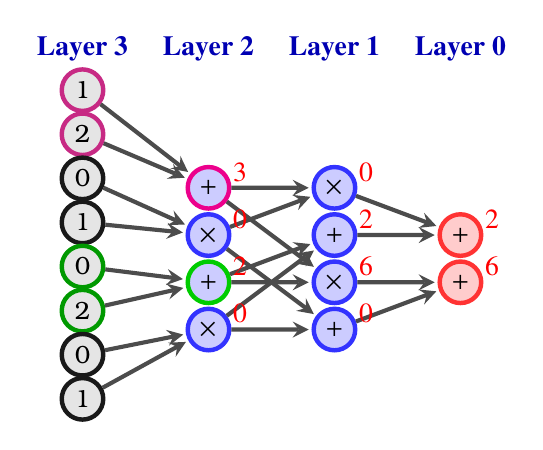
\begin{tikzpicture}[
            % Define styles for different parts of the circuit
            input/.style={circle, ultra thick, draw=gray!20!black, fill=gray!20, minimum size=15pt, inner sep=0pt},
            gate/.style={circle, ultra thick, draw=blue!80, fill=blue!20, minimum size=15pt, inner sep=0pt},
            output/.style={circle, ultra thick, draw=red!80, fill=red!20, minimum size=15pt, inner sep=0pt},
            conn/.style={-stealth, draw=black!70, shorten >=1pt, line width=1.5pt},
            scale=0.8
        ]

        % --- Layer Labels ---
        \node[font=\bfseries, align=center] at (0, 7.45) {\textcolor{blue!70!black}{Layer 3}};
        \node[font=\bfseries, align=center] at (2, 7.45) {\textcolor{blue!70!black}{Layer 2}};
        \node[font=\bfseries, align=center] at (4, 7.45) {\textcolor{blue!70!black}{Layer 1}};
        \node[font=\bfseries, align=center] at (6, 7.45) {\textcolor{blue!70!black}{Layer 0}};

        % --- Layer 0: Input Nodes (8) ---
        % We use a \foreach loop to create the 8 input nodes vertically
        \node[input, draw=magenta!80!black] (l0-1) at (0, 7.5 - 0.7*1) {$\xval{1}$};
        \node[input, draw=magenta!80!black] (l0-2) at (0, 7.5 - 0.7*2) {$\xval{2}$};
        \node[input] (l0-3) at (0, 7.5 - 0.7*3) {$\xval{3}$};
        \node[input] (l0-4) at (0, 7.5 - 0.7*4) {$\xval{4}$};
        \node[input, draw=green!60!black] (l0-5) at (0, 7.5 - 0.7*5) {$\xval{5}$};
        \node[input, draw=green!60!black] (l0-6) at (0, 7.5 - 0.7*6) {$\xval{6}$};
        \node[input] (l0-7) at (0, 7.5 - 0.7*7) {$\xval{7}$};
        \node[input] (l0-8) at (0, 7.5 - 0.7*8) {$\xval{8}$};
        % \foreach \i in {1,...,8} {
        %     \node[input] (l0-\i) at (0, 7.5 - 0.7*\i) {$\xval{\i}$};
        % }

        % --- Layer 1: Gate Nodes (4) ---
        % Alternating between + and x gates
        \node[gate, draw=magenta] (l1-1) at (2, 5.25) {$+$};

        \node[gate] (l1-2) at (2, 4.5) {$\times$};
 
        \node[gate, draw=green!80!black] (l1-3) at (2, 3.75) {$+$};

        \node[gate] (l1-4) at (2, 3.0) {$\times$};

        % --- Layer 2: Gate Nodes (4) ---
        \node[gate] (l2-1) at (4, 5.25) {$\times$};
        \node[gate] (l2-2) at (4, 4.5) {$+$};
        \node[gate] (l2-3) at (4, 3.75) {$\times$};
        \node[gate] (l2-4) at (4, 3.0) {$+$};

        % --- Layer 3: Output Nodes (2) ---
        \node[output] (l3-1) at (6, 4.5) {$+$};
        \node[output] (l3-2) at (6, 3.75) {$+$};


        % --- Connections ---

        % Connections from Layer 0 to Layer 1
        \foreach \i in {1,...,4} {
            \pgfmathtruncatemacro{\j}{2 * \i - 1} % Calculate first source node index
            \pgfmathtruncatemacro{\k}{2 * \i}     % Calculate second source node index
            \draw[conn] (l0-\j) -- (l1-\i);
            \draw[conn] (l0-\k) -- (l1-\i);
        }

        % Connections from Layer 1 to Layer 2
        % This wiring pattern creates a mixing of the signals
        \draw[conn] (l1-1) -- (l2-1);
        \draw[conn] (l1-2) -- (l2-1);

        \draw[conn] (l1-3) -- (l2-2);
        \draw[conn] (l1-4) -- (l2-2);

        \draw[conn] (l1-1) -- (l2-3);
        \draw[conn] (l1-3) -- (l2-3);

        \draw[conn] (l1-2) -- (l2-4);
        \draw[conn] (l1-4) -- (l2-4);

        % Connections from Layer 2 to Layer 3
        \draw[conn] (l2-1) -- (l3-1);
        \draw[conn] (l2-2) -- (l3-1);

        \draw[conn] (l2-3) -- (l3-2);
        \draw[conn] (l2-4) -- (l3-2);

        % Values in gates, layer 2
        \node at (2.5, 5.5) {\textcolor{red}{3}};
        \node at (2.5, 4.75) {\textcolor{red}{0}};
        \node at (2.5, 4.0) {\textcolor{red}{2}};
        \node at (2.5, 3.25) {\textcolor{red}{0}};

        % Values in gates, layer 1
        \node at (4.5, 5.5) {\textcolor{red}{0}};
        \node at (4.5, 4.75) {\textcolor{red}{2}};
        \node at (4.5, 4.0) {\textcolor{red}{6}};
        \node at (4.5, 3.25) {\textcolor{red}{0}};

        % Values in gates, layer 0
        \node at (6.5, 4.75) {\textcolor{red}{2}};
        \node at (6.5, 4.0) {\textcolor{red}{6}};
        \end{tikzpicture}
        \end{center}
        \vspace{-12.5px}
        \begin{gather*}
        \mathsf{add}_2 \; \text{is non-zero}: (\textcolor{magenta}{(0,0)},\textcolor{magenta!80!black}{(0,0,0)},\textcolor{magenta!80!black}{(0,0,1)}), 
        \;
        (\textcolor{green!80!black}{(1,0)},\textcolor{green!60!black}{(1,0,0)},\textcolor{green!60!black}{(1,0,1)}). \\
        \widetilde{\mathsf{add}}_2(\mathbf{X},\mathbf{Y},\mathbf{Z}) = (1-X_1)(1-X_2)(1-Y_1)(1-Y_2)(1-Y_3)(1-Z_1)(1-Z_2)Z_3
        \end{gather*}
    \end{frame}

    \begin{frame}{Reducing to Sum-Check}
        \begin{block}{Remark}
            Note that the operations encodings $\mathsf{add}_i$ and
            $\mathsf{mul}_i$ (and thus MLEs $\widetilde{\mathsf{add}}_i$ and
            $\widetilde{\mathsf{mul}}_i$) do not depend on the solution witness
            $\{\mathbf{x}^{\langle i \rangle}\}_{i \in [d+1]}$, while the gates
            encodings $W_i$ do depend.
        \end{block}

        \textbf{Idea:} Prover sends the claimed value of $\widetilde{W}_0$ (say,
        $D: \{0,1\}^{v_0} \to \mathbb{F}$), then reduce the claim to the next
        around with $\widetilde{W}_1$ (in general, prove the reducing from
        $\widetilde{W}_i$ to $\widetilde{W}_{i+1}$). 
        \begin{figure}
            
\includegraphics[width=0.6\textwidth]{images/lecture_16/where.png}
        \end{figure}
    \end{frame}

    \begin{frame}{Sum-Check Protocol Applied}
        \begin{figure}
            
\includegraphics[width=0.3\textwidth]{images/lecture_16/dicaprio.jpg}
        \end{figure}

        \begin{lemma}
        The following statement holds:
        \begin{align*}
            \widetilde{W}_i(\mathbf{z}) = \sum_{\boldsymbol{b},\boldsymbol{c} \in \{0,1\}^{v_{i+1}}} &\Big[ \widetilde{\mathsf{add}}_i(\mathbf{z},\boldsymbol{a},\boldsymbol{b})(\widetilde{W}_{i+1}(\boldsymbol{b}) + \widetilde{W}_{i+1}(\boldsymbol{c})) \\
            &+ \widetilde{\mathsf{mul}}_i(\mathbf{z},\boldsymbol{b},\boldsymbol{c})\widetilde{W}_{i+1}(\boldsymbol{b})\widetilde{W}_{i+1}(\boldsymbol{c})\Big].
        \end{align*}
        \end{lemma}
    \end{frame}

    \begin{frame}{Why Lemma works?}
        Both sides are multilinear polynomials, thus it suffices to check the equality only over the 
        boolean hypercube $\mathbf{z} \in \{0,1\}^{v_i}$.

        Fix $\mathbf{z}=\mathbf{z}_0 \in \{0,1\}^{v_i}$. Without loss of generality, assume
        $\mathbf{z}_0$ is the addition gate. This way, we reduced the check to:
        \begin{equation*}
            \widetilde{W}_i(\mathbf{z}_0) = \sum_{\boldsymbol{b},\boldsymbol{c} \in \{0,1\}^{v_{i+1}}} \widetilde{\mathsf{add}}_i(\mathbf{z},\boldsymbol{a},\boldsymbol{b})(\widetilde{W}_{i+1}(\boldsymbol{b}) + \widetilde{W}_{i+1}(\boldsymbol{c}))
        \end{equation*}

         According to $\widetilde{\mathsf{add}}$ definition, the only term that is not
        zero in the sum is for
        $(\boldsymbol{b},\boldsymbol{c})=(\mathsf{in}_{1,i}(\mathbf{z}_0),
        \mathsf{in}_{2,i}(\mathbf{z}_0))$. Therefore, our sum is:
        \begin{equation*}
            \widetilde{W}_i(\mathbf{z}_0) = \widetilde{W}_{i+1}(\mathsf{in}_{1,i}(\mathbf{z}_0)) + \widetilde{W}_{i+1}(\mathsf{in}_{2,i}(\mathbf{z}_0))
        \end{equation*}

        \begin{alertblock}{Key Procedure}
            Apply the Sum-Check protocol on the function 
            \begin{equation*}
                \small f_i(\boldsymbol{b}, \boldsymbol{c}; \mathbf{r}_i) = \widetilde{\mathsf{add}}_i(\mathbf{r}_i, \boldsymbol{b}, \boldsymbol{c})(\widetilde{W}_{i+1}(\boldsymbol{b}) + \widetilde{W}_{i+1}(\boldsymbol{c})) + \widetilde{\mathsf{mul}}_i(\mathbf{r}_i, \boldsymbol{b}, \boldsymbol{c})\widetilde{W}_{i+1}(\boldsymbol{b})\widetilde{W}_{i+1}(\boldsymbol{c}).
            \end{equation*}
        \end{alertblock}
    \end{frame}

    \begin{frame}{Caveat with Sum-Check}
        Note that the verifier $\mathcal{V}$ does not know $\widetilde{W}_{i+1}$.

        In fact, he does not need to until the last round, where he needs to
        call an oracle access $\mathcal{O}^{\; f_i}$ at $(\boldsymbol{b}^*,
        \boldsymbol{c}^*) \leftarrowS \mathbb{F}^{2v_{i+1}}$. 
        
        This requires evaluating:
        \begin{itemize}
            \item $\widetilde{\mathsf{add}}_i(\mathbf{r}_i,\boldsymbol{b}^*, \boldsymbol{c}^*)$ --- can be done by $\mathcal{V}$.
            \item $\widetilde{\mathsf{mul}}_i(\mathbf{r}_i,\boldsymbol{b}^*, \boldsymbol{c}^*)$ --- can be done by $\mathcal{V}$.
            \item $\widetilde{W}_{i+1}(\boldsymbol{b}^*)$ and $\widetilde{W}_{i+1}(\boldsymbol{c}^*)$ --- $\mathcal{V}$ needs $\mathcal{P}$'s assistance.
        \end{itemize}

        $\mathcal{P}$ sends two values $z_b =
        \widetilde{W}_{i+1}(\boldsymbol{b}^*)$ and $z_c =
        \widetilde{W}_{i+1}(\boldsymbol{c}^*)$.  If we had only one value to
        check, we could use the standard Sum-Check reduction, but here we have
        two randomnesses!
    \end{frame}

    \begin{frame}{Line Restriction Trick}
        \begin{block}{Proposition}
            Let $\ell: \mathbb{F} \to \mathbb{F}^{v_{i+1}}$ be the line such that
            $\ell(0)=\boldsymbol{b}^*$ and $\ell(1)=\boldsymbol{c}^*$. Then, the prover
            $\mathcal{P}$ sends the univariate polynomial $q(X)$ claimed to be equal to
            $\widetilde{W}_{i+1} \circ \ell$ --- the restriction of
            $\widetilde{W}_{i+1}$ to the line $\ell$. $\mathcal{V}$ checks whether
            indeed $\ell(0)=z_b$ and $\ell(1)=z_c$, then chooses a random point
            $\mathbf{r}^* \xleftarrow{R} \mathbb{F}^{v_{i+1}}$ and checks whether
            $\widetilde{W}_{i+1}(\ell(\mathbf{r}^*)) = q(\mathbf{r}^*)$.
        \end{block}

        This way, the interaction ends with new claim about next(previous) layer
        $\widetilde{W}_{i+1}(\mathbf{r}_{i+1})$ with
        $\mathbf{r}_{i+1}=\ell(\mathbf{r}^*)$.

        In the last round, $\mathcal{V}$ computes
        $\widetilde{W}_d(\mathbf{r}_d)$ on his own.
    \end{frame}

    \begin{frame}{Protocol Summary}
        \begin{itemize}
            \item $\mathcal{P}$ sends function $D: \{0,1\}^{v_0} \to
            \mathbb{F}$, claimed to equal $W_0$.
            \item $\mathcal{V}$ picks random $\mathbf{r}_0 \leftarrowS
            \mathbb{F}^{v_0}$ and lets $m_0 \gets \widetilde{D}(\mathbf{r}_0)$.
            \item For each round $i \in [d]$ do the following:
            \begin{itemize}
                \item Define the $2v_{i+1}$-variate polynomial:
                \vspace{-5px}
                \begin{equation*}
                    \small f_i(\boldsymbol{b}, \boldsymbol{c}; \mathbf{r}_i) = \widetilde{\mathsf{add}}_i(\mathbf{r}_i, \boldsymbol{b}, \boldsymbol{c})(\widetilde{W}_{i+1}(\boldsymbol{b}) + \widetilde{W}_{i+1}(\boldsymbol{c})) + \widetilde{\mathsf{mul}}_i(\mathbf{r}_i, \boldsymbol{b}, \boldsymbol{c})\widetilde{W}_{i+1}(\boldsymbol{b})\widetilde{W}_{i+1}(\boldsymbol{c}).
                \end{equation*}
                \item $\mathcal{P}$ claims $\sum_{\boldsymbol{b},\boldsymbol{c}
                \in \{0,1\}^{v_{i+1}}} f_i(\boldsymbol{b},\boldsymbol{c};
                \mathbf{r}_i) = m_i$.
                \item $\mathcal{P}$ and $\mathcal{V}$ interact using Sum-Check
                protocol until the last round when $\mathcal{V}$ needs to
                evalutate $f_i$ at $\boldsymbol{b}^*, \boldsymbol{c}^*
                \leftarrowS \mathbb{F}^{v_{i+1}}$.
                \item $\mathcal{P}$ and $\mathcal{V}$ compute the line $\ell:
                \mathbb{F} \to \mathbb{F}^{v_{i+1}}$ s.t.
                $\ell(0)=\boldsymbol{b}^*$ and $\ell(1)=\boldsymbol{c}^*$.
                \item $\mathcal{P}$ sends $q$ claimed to equal
                $\widetilde{W}_{i+1} \circ \ell$.
                \item $\mathcal{V}$ validates the last round of sum-check using
                $\ell(0)$ and $\ell(1)$, then chooses $\mathbf{r}^*
                \leftarrowS \mathbb{F}^{v_{i+1}}$ and sets $\mathbf{r}_{i+1}
                \gets \ell(\mathbf{r}^*)$ and $m_{i+1} \gets
                q(\mathbf{r}_{i+1})$.
                \item The check reduces to verifying $\widetilde{W}_{i+1}(\mathbf{r}_{i+1})=m_{i+1}$.
            \end{itemize}
            \item $\mathcal{V}$ directly checks whether
            $m_d=\widetilde{W}_d(\mathbf{r}_d)$.
        \end{itemize}
    \end{frame}

    \section{Grand Product Check}

    \begin{frame}{Grand Product Relation}
        \begin{equation*}
        \mathcal{R}_{GP} = \big\{ (p \in \mathbb{F}, \mathbf{v} \in \mathbb{F}^m)\colon p = \prod_{i=0}^m v_i \big\} \label{grand-product-relation}
        \end{equation*}
        Assume that $m$ is a power of $2$.

        
        
        Let $\widetilde{v}$ be an MLE of $\mathbf{v}$, by viewing $\mathbf{v}$ as a 
        function mapping $\{0,1\}^{\log m} \rightarrow \mathbb{F}$.
    \end{frame}

    \begin{frame}{Main Lemma}
        \begin{lemma}
        A scalar $p$ and a vector $\mathbf{v}$ satisfies the relation $\mathcal{R}_{GP}$ if and only if there exists a 
        multilinear polynomial $f$ in $\log m + 1$ variables such that $f(1,\dots,1, 0) = p$ and $\forall x \in \{0,1\}^{\log m}$
        the following hold:
        \begin{gather*}
        f(0, x) = v(x)\\
        f(1,x) = f(x, 0) \cdot f(x, 1)
        \end{gather*}
        Such polynomial $f$ has the following construction: \begin{itemize}
            \item $f(1,\dots,1) = 0$
            \item For all $\ell \in [\log m]$ and $x \in \{0,1\}^{\log m - \ell}$: \\ 
            \vspace{-0.8em}
            \begin{equation*}
                f(1^\ell, 0, x) = \prod_{y \in \{0,1\}^\ell}v(x,y)
            \end{equation*}
        \end{itemize}
        \end{lemma}
    \end{frame}

    \begin{frame}
        \begin{example}
            Let $m=4$ ($\log m=2$), $\mathbf{v} = \{1, 2, 3, 4\}$, consequently $p = 1\times2\times3\times4=24$, then:
            \vspace{-5px}
            
            \begin{align*}
            v(x_1, x_2)& = 1 + 2x_1 + x_2\\
            v(x_1,x_2)&: \quad v(0,0)=1,\; v(0,1)=2,\; v(1,0)=3,\; v(1,1)=4.
            \vspace{-5px}
            \end{align*}
            
            Now, we define $f$ as follows:
            \vspace{-5px}
            \begin{equation*}
                f(0,0,0)= 1,\; f(0,0,1)=2,\; f(0,1,0)=3,\; f(0,1,1)=4,
                \vspace{-5px}
            \end{equation*}
            
            and:
            \vspace{-10px}
            \begin{align*}
            f(1,0,0)&= f(0,0,0) \times f(0,0,1) = 1 \times 2 = 2,\\ 
            f(1,0,1)&= f(0,1,0) \times f(0,1,1) = 3 \times 4 = 12,\\ 
            f(1,1,0)&= f(1,0,0) \times f(1,0,1) = 2 \times 12 = 24 = p,\\ 
            f(1,1,1)&= 0.
            \vspace{-5px}
            \end{align*}
        \end{example}
    \end{frame}

    \begin{frame}
        \begin{example}
            \begin{center}
                \scalebox{1.0}{
                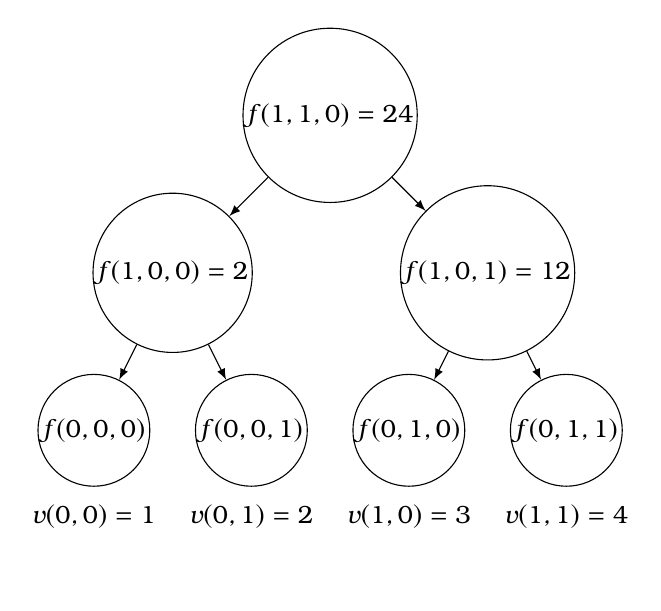
\begin{tikzpicture}[
                    level 1/.style={level distance=2cm, sibling distance=4cm},
                    level 2/.style={level distance=2cm, sibling distance=2cm},
                    level 3/.style={level distance=1.1cm, sibling distance=2cm, edge from parent/.style={draw=none},},
                    edge from parent/.style={draw, -latex},
                    every node/.style={circle,draw,inner sep=1pt}
                ]
                \node {$f(1,1,0)=24$}
                    child {
                        node {$f(1,0,0)=2$}
                        child { node {$f(0,0,0)$}
                            child { node[draw=none] {$\displaystyle v(0,0)=1$} }
                        }
                        child { node {$f(0,0,1)$}
                            child { node[draw=none] {$\displaystyle v(0,1)=2$} }
                        }
                    }
                    child {
                        node {$f(1,0,1)=12$}
                        child { node {$f(0,1,0)$}
                            child { node[draw=none] {$\displaystyle v(1,0)=3$} }
                        }
                        child { node {$f(0,1,1)$}
                            child { node[draw=none] {$\displaystyle v(1,1)=4$} }
                        }
                    };
                \end{tikzpicture}
                }
            \end{center}
            \vspace{-15px}
        \end{example}
    \end{frame}

    \begin{frame}{Where Is Sum-Check?}
        \centering
        % Adjust width or height as needed:
        
\includegraphics[width=1\linewidth]{./images/lecture_17/where-is-everyone.png}
        \label{fig:meme}
    \end{frame}

    \begin{frame}{Zero-Check}
        \begin{equation*}
            \forall x \in \{0,1\}^{\log m}\colon f(1,x) = f(x, 0) \cdot f(x, 1)
        \end{equation*}
        
        \vspace{-10px}
        \begin{equation*}
            \forall x \in \{0,1\}^{\log m}\colon f(1,x) - f(x, 0) \cdot f(x, 1) = 0
        \end{equation*}
        
        One can use the sum-check protocol to prove the evaluation of $g$ that is referred to a MLE of $f(1,x) - f(x, 0) \cdot f(x, 1)$:
        \begin{equation*}
            g(t) = \sum_{x \in \{0,1\}^{\log m}} \widetilde{\text{eq}}(t,x) \cdot (f(1,x) - f(x, 0) \cdot f(x, 1))
        \end{equation*}
        
        By the Schwartz–Zippel lemma, for random $\tau \in \mathbb{F}^{\log m}$,
        $g(\tau) = 0$ if and only if $g = 0$, except for a soundness error of $\frac{\log m}{|\mathbb{F}|}$.
    \end{frame}

    \begin{frame}
        Thus, to prove the existence of $f$ and hence the grand product relationship, it suffices
        to prove, for some verifier selected random $\tau, \gamma \in \mathbb{F}^\ell$, that:
        \begin{gather}
        \label{eq:grands0}
            0 = \sum_{x \in \{0,1\}^{\log m}} \widetilde{\text{eq}}(x, \tau) \cdot (f(1,x) - f(x, 0) \cdot f(x, 1))\\
        \label{eq:grands1}
            f(0, \gamma) = \widetilde{v}(\gamma)\\
        \label{eq:grands2}
            f(1,\dots,1, 0) = p
        \end{gather}
    \end{frame}

    \begin{frame}
        \begin{algorithm}[H]
            \caption{Grand Product Check}\label{alg:sum_check_grand_product}
            \DontPrintSemicolon
            \SetAlgoLined

            \textbf{$\mathcal P$:}
            Compute polynomials 
            $v\in\mathbb{F}^{\log m}[x]$, 
            $f\in\mathbb{F}^{\log m+1}[x]$ 
            such that
            \vspace{-1em}
            \begin{equation*}
                \vspace{-1.6em}
                p = \prod_{x\in\{0,1\}^{\log m}} v(x)
                \quad\text{and}\quad
                f, v \text{ satisfy }(\ref{eq:grands0}),\,(\ref{eq:grands1}),\,(\ref{eq:grands2}).
                \vspace{-5px}
            \end{equation*}\;

            \textbf{$\mathcal P$:}
            $C_f \leftarrow \textsc{Commit}(f)$;
            $C_v \leftarrow \textsc{Commit}(v)$;
            send $C_f, C_v$ to $\mathcal V$.\;

            \textbf{$\mathcal V$:}
            Choose random $\tau,\gamma\in\mathbb{F}^{\log m}$ and send them to $\mathcal P$.\;

            \textbf{$\mathcal P$:}
            Compute $g(x)\;=\;\widetilde{\mathrm{eq}}(x,\tau)\,\bigl(f(1,x)-f(x,0)\,f(x,1)\bigr).$

            \textbf{$\mathcal P$ \& $\mathcal V$:}
            Run \textsc{SumCheckProtocol}($0,\;g,\;C_f$)

            \textbf{$\mathcal V$:}
            $a \leftarrow \textsc{Query}(C_f,(0,\gamma)), \;$ $v(\gamma)\leftarrow \textsc{Query}(C_v,\gamma)$.\;
            \If{$a \neq v(\gamma)$}{
                \textbf{$\mathcal V$ rejects}.\;
            }

            \textbf{$\mathcal V$:}
            $r \leftarrow \textsc{Query}(C_f,(1,\dots,1,0))$.\;
            \If{$r \neq p$}{
                \textbf{$\mathcal V$ rejects}.\;
            }
        \end{algorithm}
    \end{frame}

    \section{Randomized Permutation Check}

    \begin{frame}
        The goal is to verify, with high probability, whether two sequences of tuples
        are permutations of each other, without performing a full sort or pairwise comparison.

        
        \begin{equation*}
        A = \{(1,2,3),\,(4,0,6)\}, \quad
        B = \{(4,0,6),\,(1,2,3)\}.
        \end{equation*}
        \textit{The naive approach would be to sort both sequences and then compare them.}
    \end{frame}

    \begin{frame}{Reed-Solomon Fingerprinting}
        \begin{definition}[Reed-Solomon Fingerprinting]
            Let $\mathbf{a} \in \mathbb{F}^{n}$, then for a random $\gamma \in \mathbb{F}$, the Reed-Solomon 
            fingerprinting of $\mathbf{a}$ is defined as:
            \begin{equation*}
                h_{\gamma}(\mathbf{a}) = \sum_{i \in n} a_i \cdot \gamma^i.
            \end{equation*}

            
            $h_{\gamma}(\mathbf{a})$ uniquely identifies the sequence $\mathbf{a}$ with high probability,
            i.e., \\let $\mathbf{b} \in F^n$ and $\mathbf{a} \neq \mathbf{b}$, then, according to the Schwartz-Zippel lemma:
            \begin{equation*}
                \Pr[h_{\gamma}(\mathbf{a}) = h_{\gamma}(\mathbf{b})] \leq \frac{n}{|\mathbb{F}|}.
            \end{equation*}
        \end{definition}
    \end{frame}

    \begin{frame}{Reed-Solomon Fingerprinting}
        \begin{example}
            Consider all operations in $\mathbb{F}_7$, and set $n=3$, $\gamma=3$.  
            Let
            \begin{equation*}
                \mathbf{a} = (1,2,3), \quad \mathbf{b} = (4,0,6).
            \end{equation*}
            Then
            \begin{align*}
                h_{\gamma}(1,2,3) &=1\cdot3^0 + 2\cdot3^1 + 3\cdot3^2 =1 + 6 + 6 =13 \equiv 6,\\
                h_{\gamma}(4,0,6) &=4\cdot1 + 0\cdot3 + 6\cdot2 =4 + 0 + 12 =16 \equiv 2.
            \end{align*}
        \end{example}
    \end{frame}

    \begin{frame}{Randomized Permutation Check}
        \begin{definition}[Randomized Permutation Check]
            Let $A$ and $B$ be two multisets of tuples in $\mathbb{F}^n$. Define
            \begin{equation*}
                \mathcal{H}_{\tau,\gamma}(X)\;=\;\prod_{x \in X}\bigl(h_{\gamma}(x)-\tau\bigr).
            \end{equation*}
            
            Then comparing $\mathcal{H}_{\tau,\gamma}(A)$ and $\mathcal{H}_{\tau,\gamma}(B)$ yields a
            randomized test for whether $A$ and $B$ are permutations of one another. Concretely:
            \begin{itemize}
                \item (Completeness) If $A=B$ (as multisets), then  
                    \vspace{-5px}
                    \begin{equation*}
                        \mathcal{H}_{\tau,\gamma}(A)=\mathcal{H}_{\tau,\gamma}(B)
                        \vspace{-5px}
                    \end{equation*}
                    with probability 1 over uniform $\tau,\gamma\in\mathbb{F}$.
                \item (Soundness) If $A\neq B$, then
                    \vspace{-5px}
                    \begin{equation*}
                        \Pr\left[\,\mathcal{H}_{\tau,\gamma}(A)=\mathcal{H}_{\tau,\gamma}(B)\right]\;\le\; \frac{\max(|A|,|B|)}{|\mathbb{F}|}.
                    \end{equation*}
            \end{itemize}
        \end{definition}
    \end{frame}

    \begin{frame}
        \begin{example}
            Consider all operations in $\mathbb{F}_7$, set $n=3$, $\tau=5$, and $\gamma=3$.\\
            Let $A = \{(1,2,3),\,(4,0,6)\}, \quad B = \{(4,0,6),\,(1,2,3)\}.$
            
            
            \vspace{5px}
            First compute the Reed–Solomon fingerprints modulo 7:
            \vspace{-7px}
            \begin{align*}
                h_{\gamma}(1,2,3) &=1\cdot3^0 + 2\cdot3^1 + 3\cdot3^2 =1 + 6 + 6 =13 \equiv 6,\\
                h_{\gamma}(4,0,6) &=4\cdot1 + 0\cdot3 + 6\cdot2 =4 + 0 + 12 =16 \equiv 2. \\[-23pt]
            \end{align*}
            
            Now form the shifted products:
            \vspace{-7px}
            \begin{align*}
                \mathcal{H}_{\tau,\gamma}(A) &=(6-5)\,(2-5) =1\cdot(-3)\equiv4,\\
                \mathcal{H}_{\tau,\gamma}(B) &=(2-5)\,(6-5) =(-3)\cdot1\equiv4,\\[-23pt]
            \end{align*}
            so the test \emph{accepts} $A$ vs.\ $B$ (they are indeed permutations). \\
            
            
            \vspace{5px}
            Now consider a non-permutation $B' = \{(1,2,3),\,(2,1,3)\}.$
            \vspace{-5px}
            \begin{equation*}
                h_{\gamma}(2,1,3) =2\cdot1 + 1\cdot3 + 3\cdot2 =2 + 3 + 6 =11 \equiv 4.
                \vspace{-10px}
            \end{equation*}
            \begin{equation*}
                \mathcal{H}_{\tau,\gamma}(B') =(6-5)\,(4-5) =1\cdot(-1)\equiv6\neq4,
                \vspace{-5px}
            \end{equation*}
            so the test \emph{rejects} $A$ vs.\ $B'$.  
        \end{example}
    \end{frame}

    \section{Offline Memory Checking}

    \begin{frame}{Motivation}
        Consider Alice, who stores two values on Bob's dedicated server at 
        addresses $0$ and $1$.  Initially, Bob's memory contains
        \vspace{-6px}
        \begin{equation*}
            M \;=\;\{(0,100),\;(1,200)\}.
            \vspace{-6px}
        \end{equation*}
        Alice then performs the following operations in sequence:
        
        \begin{enumerate}
            \item writes $150$ at address $0$.  Bob updates his memory to $\{(0,150),(1,200)\}$. 
            
            \vspace{-3px}
            \item read from address $0$ and obtains the reply $150$.
            
            \vspace{-3px}
            \item reads from address $1$ and (honestly) obtains $200$.
        \end{enumerate}

        
        However, Bob can cheat on the very last step by returning a wrong value:
        \begin{equation*}
            (1,200)\;\longrightarrow\;(1,300).
            \vspace{-5px}
        \end{equation*}

        
        Without keeping an auditable record of all reads, Alice cannot later prove that all 
        replies came from correct memory contents.
    \end{frame}

    \begin{frame}{Memory Model}
        Each \textbf{memory cell} can be described as a tuple $\mathsf{(addr, val, counter)}$.
        \begin{itemize}
            \item $\mathsf{addr}$ is the address of the memory cell;
            \vspace{-5px}
            \item $\mathsf{val}$ is the value stored at that address;
            \vspace{-5px}
            \item $\mathsf{counter}$ is a counter that is incremented each time the value at that address is written to.
        \end{itemize}

        

        \vspace{5px}
        The protocol utilizes four sets of tuples:
        \begin{itemize}
            \item $\mathbf{init}$ -- contains the initial memory state;
            \vspace{-5px}
            \item $\mathbf{write}$ -- contains memory cels that represent write operations;
            \vspace{-5px}
            \item $\mathbf{read}$ -- contains memory cels that represent read operations;
            \vspace{-5px}
            \item $\mathbf{final}$ -- contains the final memory state, where all counters are set to the last value.
        \end{itemize}
    \end{frame}

    \begin{frame}{Memory Operations}
        \begin{itemize}
            \item \textbf{Init:} load initial state; all counters = 0;  
            \item \textbf{Read:}  
            \begin{itemize}
                \item Query untrusted memory at \textsf{addr} → \textsf{(val,counter)};  
                \item Append \textsf{(addr,val,counter)} to \textbf{reads};
                \item Append \textsf{(addr,val,counter+1)} to \textbf{writes}.
            \end{itemize}
            \item \textbf{Write:} 
            \begin{itemize}
                \item Query untrusted memory at \textsf{addr} → \textsf{(val,counter)};  
                \item Append \textsf{(addr,val,counter)} to \textbf{reads};
                \item Append \textsf{(addr,\textbf{newval},counter+1)} to \textbf{writes}.
            \end{itemize}
        \end{itemize}
    \end{frame}

    \begin{frame}{Consistency Check}
        After all reads and writes are done, the $\mathbf{final}$ set is populated with the final memory state. 

        \begin{lemma}
            One can check the consistency of the memory operations by verifying that:
            \begin{equation*}
                \mathbf{read} \cup \mathbf{final} = \mathbf{write} \cup \mathbf{init}.
                \vspace{-5px}
            \end{equation*}
            Equivalently, via randomized permutation check:
            \vspace{-5px}
            \begin{equation*}
                \mathcal{H}_{\tau,\gamma}(\mathbf{read}) \cdot \mathcal{H}_{\tau,\gamma}(\mathbf{final}) = 
                \mathcal{H}_{\tau,\gamma}(\mathbf{write}) \cdot \mathcal{H}_{\tau,\gamma}(\mathbf{init}).
            \end{equation*}
        \end{lemma}
    \end{frame}

    \begin{frame}
        \begin{example}
            Suppose the initial memory is:
            \vspace{-5px}
            \begin{equation*}
                \mathbf{init} =\{(0,2,0), \; (1,5,0), \; (2,7,0), \; (3,9,0)\},
                \vspace{-5px}
            \end{equation*}
            while $\mathbf{read} = \varnothing \; \text{and} \; \mathbf{write} = \varnothing$.

            
            \vspace{6px}
            \begin{center}
                \begin{tabular}{c|c|c|c}
                \textbf{step} & \textbf{operation} & $\Delta\mathbf{read}_{\text{step}}$ & $\Delta\mathbf{write}_{\text{step}}$\\\hline
                1 & read(1)$  \; \to \; (5, 0)$ & $(1,5,0)$ & -        \\
                2 & write((1,6))                & -         & $(1,6,1)$\\
                3 & read(2)$  \; \to \; (7, 0)$ & $(2,7,0)$ & -        \\
                4 & write((2,7))                & -         & $(2,7,1)$\\
                \end{tabular}
            \end{center}
            
            \vspace{5px}
            \begin{equation*}
                \mathbf{read} = \{(1,5,0), \; (2,7,0)\},\quad
                \mathbf{write} = \{(1,6,1), \; (2,7,1)\}
                \vspace{-5px}
            \end{equation*}
            \begin{equation*}
                \mathbf{final} = \{(0,2,0), \; (1,6,1), \; (2,7,1), \; (3,9,0)\}
            \end{equation*}
            
            One can clearly see that $\mathbf{read} \cup \mathbf{final} = \mathbf{write} \cup \mathbf{init}$.
            \vspace{-5px}
            \begin{align*}
                \{\textcolor{blue}{\mathbf{(1,5,0), (2,7,0)}}\} &\cup \{(0,2,0), \textcolor{red}{\mathbf{(1,6,1), (2,7,1)}}, (3,9,0)\} = \\
                = \{\textcolor{red}{\mathbf{(1,6,1), (2,7,1)}}\} &\cup \{(0,2,0), \textcolor{blue}{\mathbf{(1,5,0), (2,7,0)}}, (3,9,0)\}
            \end{align*}
        \end{example}
    \end{frame}

    \begin{frame}
        \begin{example}
            Suppose the initial memory is:
            \vspace{-5px}
            \begin{equation*}
                \mathbf{init} =\{(0,2,0), \; (1,5,0), \; (2,7,0), \; (3,9,0)\},
                \vspace{-5px}
            \end{equation*}
            while $\mathbf{read} = \varnothing \; \text{and} \; \mathbf{write} = \varnothing$.

            
            \vspace{6px}
            \begin{center}
                \begin{tabular}{c|c|c|c}
                \textbf{step} & \textbf{operation} & $\Delta\mathbf{read}_{\text{step}}$ & $\Delta\mathbf{write}_{\text{step}}$\\\hline
                1 & read(1)$  \; \to \; (a, 0)$ & $(1,a,0)$ & -        \\
                2 & write((1,6))                & -         & $(1,6,1)$\\
                \end{tabular}
            \end{center}
            
            \vspace{5px}
            \begin{equation*}
                \mathbf{read} = \{(1,a,0)\},\quad
                \mathbf{write} = \{(1,6,1)\},
                \vspace{-5px}
            \end{equation*}
            \begin{equation*}
                \mathbf{final} = \{(0,2,0), \; (1,6,1), \; (2,7,1), \; (3,9,0)\}
            \end{equation*}
            
            The verifier checks $\mathbf{read} \cup \mathbf{final} = \mathbf{write} \cup \mathbf{init}$:
            \vspace{-5px}
            \begin{align*}
                \{(1,a,0)\} &\cup \{(0,2,0), (1,6,1), (2,7,0), (3,9,0)\} \neq \\
                \neq \{(1,6,1)\} &\cup \{(0,2,0), (1,5,0), (2,7,0), (3,9,0)\} \\[-20px]
            \end{align*}
            and \emph{rejects}.
        \end{example}
    \end{frame}

    \begin{frame}[plain, standout]
        \centering
        \LARGE
        \textbf{Thank you for your attention} \\
        
        \vspace{0.2cm} \Huge \ding{170} \large \\
        
        \vspace{1cm}
  
        \href{https://zkdl-camp.github.io/}{\raisebox{-.1em}{\hspace{.025em}\faIcon{globe}}\hspace{.325em}zkdl-camp.github.io} \\
  
        \href{https://github.com/ZKDL-Camp}{\raisebox{-.1em}{\hspace{.025em}\faIcon{github}}\hspace{.325em}github.com/ZKDL-Camp}
        
        \begin{center}
            
\includegraphics[width=0.15\textwidth]{images/logo.png}
        \end{center}
    \end{frame}
\end{document}
